% ex: ts=2 sw=2 sts=2 et filetype=tex
% SPDX-License-Identifier: CC-BY-SA-4.0
\begin{frame}
    \frametitle{Contenido}
    \tableofcontents
\end{frame}

\section{Bienvenida}

\begin{frame}[c]{Sobre la materia}

  Bienvenidos a la clase de \textbf{Análisis y Diseño de Algoritmos}

  \vspace{\baselineskip}
  \begin{description}
    \pausa
    \item[Horario:] Iniciamos a las \textbf{7:10 a.m.} y terminamos a las
      \textbf{9:40 a.m.}
    \pausa
    \item[Modalidad:] A distancia y \textbf{sincrónica}, o en su defecto
      en el \textbf{Laboratorio LIA} del edificio de Sistemas.
  \end{description}
\end{frame}

\begin{frame}[c]{Evaluación}
  \begin{itemize}
    \item Se usará la plataforma de \textbf{Google classroom} para las
      evaluaciones.
    \pausa
    \item Evaluación continua \textbf{100\%}
    \pausa
    \begin{itemize}
      \item Tareas
      \pausa
      \item Ejercicios en clase
    \end{itemize}
  \end{itemize}
\end{frame}

\section{Presentación de los asistentes}

\begin{frame}[c]{¡Hola!}

  \begin{columns}
    \column{0.8\textwidth}
      Mi nombre es: \textbf{Miguel Bernal Marin}

      \vspace{\baselineskip}
      Estudie la \underline{licenciatura en matemáticas} en la Universidad de
      Guadalajara, después ingrese a la \underline{maestría en ciencias de la
      computación} en el  Centro de Investigación y de Estudios Avanzados del
      IPN (\textbf{CINVESTAV}) unidad Guadalajara, en donde también realice
      mi \underline{doctorado en ciencias} con
    \column{0.2\textwidth}
      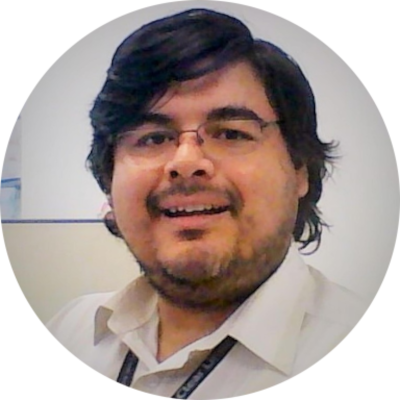
\includegraphics[scale=0.2]{profesor.png}
  \end{columns}

  especialidad en robótica y visión computacional.

  \vspace{\baselineskip}
  Actualmente estoy trabajando en la compañía \textbf{Intel} trabajando en la
  habilitación de las nuevas características de los procesadores Intel en
  distribuciones Linux.

  \vspace{\baselineskip}
  Por mi afición a Linux mis compañeros me conocen como \textbf{miguelinux}.

\end{frame}

\begin{frame}[c]{¿De dónde vienes?}
  \begin{enumerate}
    \item ¿Cuál es tu nombre?
    \item ¿Qué carrera estudiaste?
    \item ¿A qué te dedicas?
    \item ¿Porqué decidiste estudiar una maestría?
    \item ¿Sabes programar?
    \item ¿Qué lenguaje de programación conoces?
  \end{enumerate}
\end{frame}

\section{Software para la clase}

\begin{frame}[c]{Software para la clase}
  \begin{itemize}
    \item Python
      \begin{itemize}
        \item Thonny: Python IDE for beginners
        \item Visual Studio Code (vscode)
        \item Pycharm
      \end{itemize}
    \item Git
      \begin{itemize}
        \item https://github.com/miguelinux/ayda24.git
      \end{itemize}
  \end{itemize}
\end{frame}
